\documentclass{beamer}
%	\documentclass[handout]{beamer}

\mode<presentation> {

% The Beamer class comes with a number of default slide themes
% which change the colors and layouts of slides. Below this is a list
% of all the themes, uncomment each in turn to see what they look like.

%\usetheme{default}
%\usetheme{AnnArbor}
%\usetheme{Antibes}
%\usetheme{Bergen}
%\usetheme{Berkeley}
%\usetheme{Berlin}
%\usetheme{Boadilla}
%\usetheme{CambridgeUS}
%\usetheme{Copenhagen}
%\usetheme{Darmstadt}
%\usetheme{Dresden}
%\usetheme{Frankfurt}
%\usetheme{Goettingen}
%\usetheme{Hannover}
%\usetheme{Ilmenau}
%\usetheme{JuanLesPins}
%\usetheme{Luebeck}
\usetheme{Madrid}
%\usetheme{Malmoe}
%\usetheme{Marburg}
%\usetheme{Montpellier}
%\usetheme{PaloAlto}
%\usetheme{Pittsburgh}
%\usetheme{Rochester}
%\usetheme{Singapore}
%\usetheme{Szeged}
%\usetheme{Warsaw}

% As well as themes, the Beamer class has a number of color themes
% for any slide theme. Uncomment each of these in turn to see how it
% changes the colors of your current slide theme.

%\usecolortheme{albatross}
%\usecolortheme{beaver}
%\usecolortheme{beetle}
%\usecolortheme{crane}
\usecolortheme{dolphin}
%\usecolortheme{dove}
%\usecolortheme{fly}
%\usecolortheme{lily}
%\usecolortheme{orchid}
%\usecolortheme{rose}
%\usecolortheme{seagull}
%\usecolortheme{seahorse}
%\usecolortheme{whale}
%\usecolortheme{wolverine}

%\setbeamertemplate{footline} % To remove the footer line in all slides uncomment this line
%\setbeamertemplate{footline}[page number] % To replace the footer line in all slides with a simple slide count uncomment this line

%\setbeamertemplate{navigation symbols}{} % To remove the navigation symbols from the bottom of all slides uncomment this line
}

\usefonttheme{professionalfonts}

\usepackage{slashed,graphicx,color,amsmath,amssymb,mathtools}
\usepackage{graphicx} % Allows including images
\usepackage{xeCJK}
\usepackage{booktabs} % Allows the use of \toprule, \midrule and \bottomrule in tables
\usepackage{tikz}
\usepackage{multimedia}
% \usepackage[colorlinks,linkcolor=red]{hyperref}

\newcommand{\stuname}{学生}

%----------------------------------------------------------------------------------------
%	TITLE PAGE
%----------------------------------------------------------------------------------------

\title[波与光学]{马正物理学讲义\\波与光学篇}

\author{马正} % Your name
\institute[渊学通教育] % Your institution as it will appear on the bottom of every slide, may be shorthand to save space
{
渊学通教育广州校区 \\ % Your institution for the title page
\medskip
\textit{zs05322001@hotmail.com} % Your email address
}
\date{\today} % Date, can be changed to a custom date

\begin{document}

% \AtBeginSection[] % Do nothing for \section*
% {
%	\begin{frame}<beamer>
%		\frametitle{课程结构}
%		\tableofcontents[currentsection]
%	\end{frame}
%}

\AtBeginSubsection[] % Do nothing for \subsection*
{
	\begin{frame}<beamer>
	\frametitle{课程结构}
	\tableofcontents[currentsection, currentsubsection]
\end{frame}
}

\begin{frame}
\titlepage 
\end{frame}

\section{振动与波}

\subsection{简谐运动}

\begin{frame}{Simple Harmonic Motion 简谐运动}
	\begin{block}{简谐运动的形象(动画)}
		\begin{center}
		\href{run:./LectureNotePics/vertoscillator.gif}{\resizebox{.4\textwidth}{!}{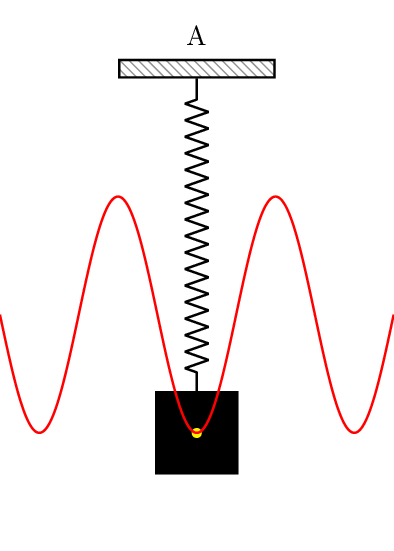
\includegraphics{./LectureNotePics/vertoscillator.png}\unskip}}\\
		\end{center}
	\end{block}
\end{frame}

\begin{frame}{Spring-Mass System 弹簧振子}
	\begin{center}
		\resizebox{.5\textwidth}{!}{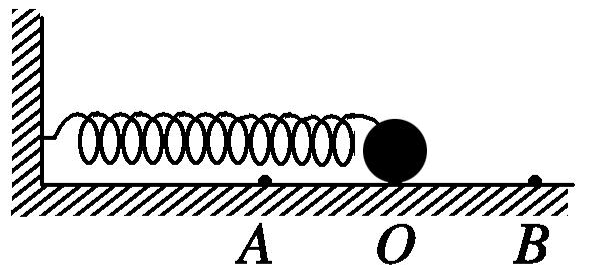
\includegraphics{./LectureNotePics/SpringMass.png}\unskip}
	\end{center}
	\begin{itemize}
		\item Hooke's Law: $F = -kx$
		\item Newton's Second Law: $F = ma$
		\item $a = \dfrac{dv}{dt} = \dfrac{d^2 x}{dt^2}$
		\item $m\dfrac{d^2 x}{dt^2} = -kx$
	\end{itemize}
\end{frame}

\begin{frame}{Spring-Mass System 弹簧振子}
	\begin{itemize}
		\item $m\dfrac{d^2 x}{dt^2} = -kx$
		\item 角频率 (angular frequency): $\omega^2 = \dfrac{k}{m}$
		\item $\dfrac{d^2 x}{dt^2} + \omega^2 x = 0$
		\item 常微分方程 (ordinary differential equation)
		\item 通解 (general solution) 与特解 (particular solution)
	\end{itemize}
\end{frame}

\begin{frame}{Spring-Mass System 弹簧振子}
	\begin{block}{通解}
		\[x\left(t\right) = C_1 \cos \omega t + C_2 \sin \omega t\]
		\[\Downarrow\]
		\[x\left(t\right) = A \cos \left(\omega t + \phi_0\right)\]
	\end{block}
	\begin{itemize}
		\item 振幅 (amplitude): $A = \sqrt{C_1^2 + C_2^2}$
		\item 相位常数 (phase constant):$\tan \phi_0 = \dfrac{C_2}{C_1}$
	\end{itemize}
\end{frame}

\begin{frame}{Spring-Mass System 弹簧振子}
	\begin{itemize}
		\item $v = \dfrac{dx}{dt} = \omega \sqrt{A^2 - x^2}$
		\item 最大速度在经过平衡位置时取得:$v_{\rm max} = \omega A$
		\item 动能:$E_k = \dfrac{1}{2} m v^2 = \dfrac{1}{2} m \omega^2 \left(A^2 - x^2\right) = \dfrac{1}{2} k \left(A^2 - x^2\right)$
		\item (弹性)势能:$E_p = \dfrac{1}{2} k x^2$
		\item 总机械能:$E_m = E_k + E_p \equiv \dfrac{1}{2} k A^2$ 保持不变!
	\end{itemize}
\end{frame}

\begin{frame}{Initial Condition 初值条件}
	\begin{itemize}
		\item ``Initial'': when $t = 0$
		\item ``Initial Condition'': the position and velocity of the mass when we press the button on our stopwatch
		\item $x_0 = x\left(0\right) = A \cos \phi_0$
		\item $v_0 = v\left(0\right) = A\omega \sin \phi_0$
	\end{itemize}
	\begin{block}{用初值条件来决定phase constant!}
		\[\phi_0 = \tan^{-1}\left(\frac{v_0}{\omega x_0}\right)\]
	\end{block}
\end{frame}

\begin{frame}{Simple Pendulum 单摆}
	\begin{columns}
	\column{.6\textwidth}
	\begin{center}
		\resizebox{\textwidth}{!}{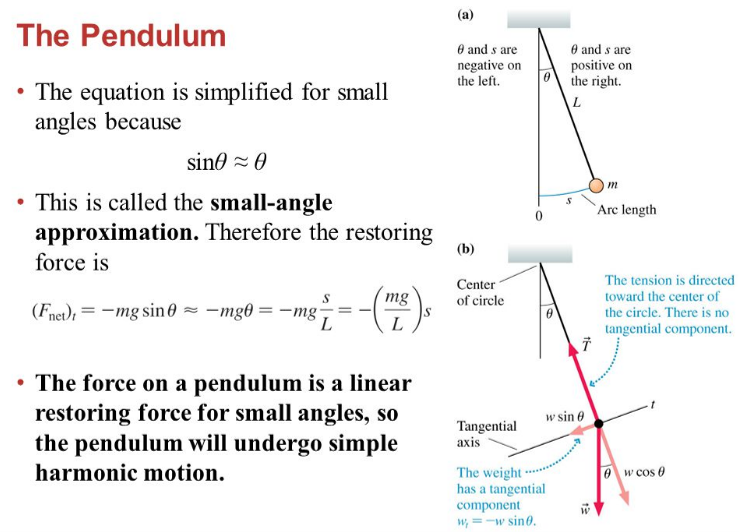
\includegraphics{./LectureNotePics/SimplePendulum.png}\unskip}
	\end{center}
	\column{.4\textwidth}
	\begin{block}{单摆的微分方程}
		\[m \frac{d^2 s}{dt^2} + \left(\frac{mg}{L}\right)s = 0\]
		\[\Downarrow\]
		\[\frac{d^2 s}{dt^2} + \left(\frac{g}{L}\right)s = 0\]
	\end{block}
	\end{columns}
	
	\medskip
	\begin{center}
		\LARGE{$\omega = \sqrt{\dfrac{g}{L}}$与摆球质量无关!}
	\end{center}
\end{frame}

\begin{frame}{单摆测量重力加速度}
	\begin{center}
		\LARGE{$g = \dfrac{4\pi^2 L}{T^2}$ 可以测量$g$}
	\end{center}

	\begin{exampleblock}{思考题}
		\begin{itemize}
			\item 一件很凑巧的事:地球表面$g \approx \pi^2 {\rm m/s}$
			\item 所以,不用计算器,口头估算:一个1米长的单摆在地球表面的周期大约是多少?
		\end{itemize}
	\end{exampleblock}
\end{frame}

\begin{frame}{SHM v.s. Uniform Circular Motion}
	\begin{block}{摩天轮上的一个吊舱(动画)}
		\begin{center}
		\href{run:./LectureNotePics/CircSHM.gif}{\resizebox{.4\textwidth}{!}{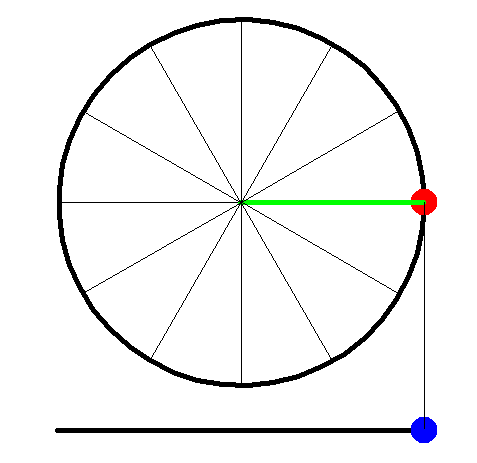
\includegraphics{./LectureNotePics/CircSHM.png}\unskip}}\\
		\end{center}
	\end{block}
	
	\begin{center}
	\begin{Large}
		匀速圆周运动的物体在侧面的投影的运动是SHM!
	\end{Large}
	\end{center}
\end{frame}

\begin{frame}{Vibration v.s. Oscillation}
	\begin{itemize}
		\item 狭义的SHM:物体相对平衡位置的位移随时间的正弦函数式的变化.
		\item 广义的SHM:任何物理量围绕一个平衡值随时间的正弦函数式变化.
	\end{itemize}
	\begin{columns}
		\column{.6\textwidth}
		\begin{center}
		\resizebox{.8\textwidth}{!}{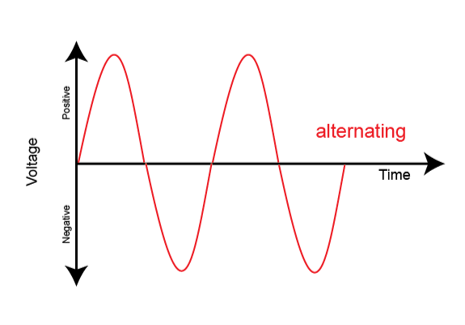
\includegraphics{./LectureNotePics/ACVoltage.png}\unskip}\\
		正弦交流电(插座里那种)
		\end{center}
		\column{.4\textwidth}
		\begin{itemize}
			\item Vibration(机械振动):物体的位置随时间的周期性变化.
			\item Oscillation(振荡):任何物理量随时间的周期性变化(包括温度、电磁场等,当然也包括vibration)
		\end{itemize}
	\end{columns}
\end{frame}

\subsection{波的基本性质}

\begin{frame}{Wave 波}
	\begin{itemize}
		\item 本质:propagation of oscillation 振荡沿一定方向的传播.
		\item 除电磁波 (electromagnetic wave) 外,所有的波都需要在介质中传播.
		\item 受到波及的每个点都围绕\textbf{各自的}平衡位置往返做SHM,所以\textbf{物质不随波传播}.
		\item 波只传播能量 (energy) 和动量 (momentum).
	\end{itemize}
\end{frame}

\begin{frame}{Sinusoidal Wave 正弦波}
	\begin{block}{正弦波的形象(动画)}
		\begin{center}
		\href{run:./LectureNotePics/Transverse.gif}{\resizebox{.6\textwidth}{!}{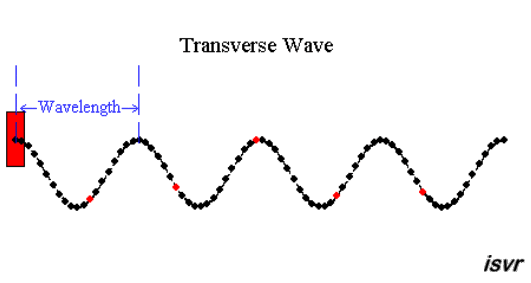
\includegraphics{./LectureNotePics/Transverse.png}\unskip}}\\
		\end{center}
	\end{block}
	
	\begin{itemize}
		\item 波上各点分别所做SHM的$\omega$、$A$都相同,不同的只有相位常数$\phi_0$
		\item 波上两点各自所做SHM的$\phi_0$的差,正比于两者沿波的传播方向的距离
	\end{itemize}
\end{frame}

\begin{frame}{Sinusoidal Wave 正弦波}
	\begin{block}{波的形象(动画)}
		\begin{center}
		\href{run:./LectureNotePics/Transverse.gif}{\resizebox{.6\textwidth}{!}{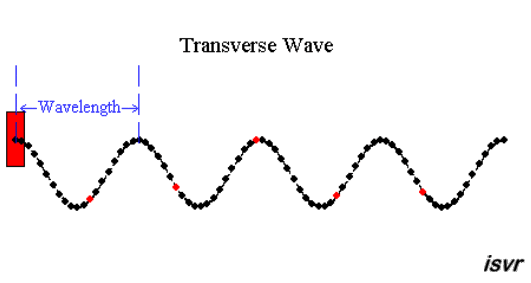
\includegraphics{./LectureNotePics/Transverse.png}\unskip}}\\
		\end{center}
	\end{block}
	
	\begin{itemize}
		\item 每个点做SHM的周期都相同,为T
		\item 波上两点的$\phi_0$差距为$2\pi$时,两点显然总是同步起伏运动的。这时两点所隔距离叫做波长 (wavelength),用$\lambda$表示.
		\item $v = \dfrac{\lambda}{T} = \lambda f$叫做波速(wave speed)
	\end{itemize}
\end{frame}

\begin{frame}{波的数学模型}
	\begin{itemize}
		\item SHM中只涉及一个点,只需描述这个点到平衡位置的位移随时间的变化即可:$y=f\left(t\right)$
		\item 波涉及介质中无数个点,必须指明每个点到各自的平衡位置的位移随时间的变化:$y=f\left(x, t\right)$
		\item 这是一个\textbf{双变量函数(function of two variables)}.
	\end{itemize}
\end{frame}

\begin{frame}{y-t and y-x graphs}
	\begin{itemize}
		\item y-t 图描述波上一个点一段时间里离开平衡位置的距离。\\图像周期 = $T$.
		\item y-x 图描述波上各个点在某一瞬间离开平衡位置的距离。\\图像周期 = $\lambda$
		\item 两种图里,图像的高度都是2倍的振幅.
	\end{itemize}
	
	\begin{center}
		\resizebox{0.5\textwidth}{!}{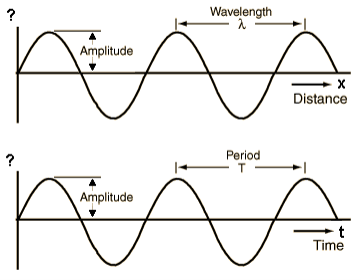
\includegraphics{./LectureNotePics/ytyxgraphs.png}\unskip}
	\end{center}
\end{frame}

\begin{frame}{Transverse v.s. Longitudinal}
	\begin{columns}
		\column{.6\textwidth}
		\begin{block}{横波与纵波(动画)}
		\begin{center}
		\href{run:./LectureNotePics/trans_longi.gif}{\resizebox{\textwidth}{!}{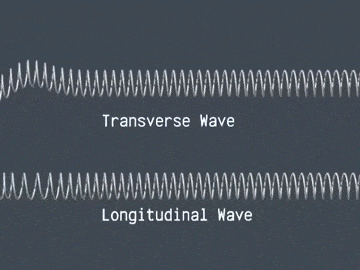
\includegraphics{./LectureNotePics/trans_longi.png}\unskip}}\\
		\end{center}
		\end{block}
		\column{.4\textwidth}
		\begin{itemize}
			\item 波上每点的往返振动沿着一个方向,而波的传播也沿着一个方向,两者没有必然联系.
			\item 如果两者相垂直,称为横波 (transverse wave).
			\item 如果两者相平行,称为纵波(longitudinal wave).
			\item 横波的典型形象是``起伏'',纵波的典型形象是``疏密''.
		\end{itemize}
	\end{columns}
\end{frame}

\begin{frame}{Pulse 脉冲}
	\begin{itemize}
		\item 单个波形在介质中的传播。
		\item 相对而言,刚才我们学的叫做连续波 (continuous wave).
		\item 脉冲其实是无数个$f$、$\lambda$不同的正弦连续波的叠加,所以它也具有波的性质,例如superposition等.
	\end{itemize}
\end{frame}

\begin{frame}{Wave Function 波函数}
	\begin{itemize}
		\item SHM的描述是:$y\left(t\right) = A \cos \left(\omega t + \phi_0\right)$
		\item 波的描述需要一个双变量函数:
	\end{itemize}
	
	\begin{block}{波函数的长相}
	\begin{itemize}
		\item 向右传播的正弦波:$y\left(x, t\right) = A \cos \left(kx \textcolor{red}{-} \omega t + \phi_0\right)$
		\item 向左传播的正弦波:$y\left(x, t\right) = A \cos \left(kx \textcolor{red}{+} \omega t + \phi_0\right)$
		\item 左正右负!
	\end{itemize}
	\end{block}
	
	\begin{itemize}
		\item $k = \dfrac{2\pi}{\lambda}$,叫做波数 (wave number)
		\item 波数越大,y-x图挤得越密集
	\end{itemize}
\end{frame}

\begin{frame}{Wave Function 波函数}
	\begin{itemize}
		\item 一般来说,某种波在某种介质中的传播速度$v$是恒定的,比如真空中光速就是$3 \times 10^8\: {\rm m/s}$,空气中声速就是$340\: {\rm m/s}$.
		\item 回忆上周的公式:$v = \lambda f$,由此可以推得:$\omega = kv$
		\item 所以正弦波的函数又可以写成:
	\end{itemize}

	\begin{block}{波函数的另一数学形式}
		\[y\left(x, t\right) = A \cos \left[k\left(x \pm vt\right) + \phi_0\right]\]
	\end{block}
\end{frame}

\begin{frame}{Partial Derivative 偏导数}
	\begin{itemize}
		\item 以前我们求导的题目中,也有字母常数.
		\item 例:$f\left(x\right) = a b x^3$,$f'\left(x\right) = 3 ab x^2$
		\item 对多变量函数求导时,先挑出一个变量,把别的变量全都看成``字母常数'',这样就把多变量变成了单变量,这样求出来的导数,叫做偏导数.
		\item 普通导数写成``$df/dx$'',偏导数写成``$\partial y/\partial x$'',其中$\partial$这个符号就是一个写得比较奇葩的字母$d$.
	\end{itemize}
\end{frame}

\begin{frame}{PDE 偏微分方程}
	\begin{itemize}
		\item 描述SHM的是关于函数$x(t)$的一条微分方程,由于所求函数是单变量,方程里含有$x(t)$的普通的导数,这种叫做常微分方程 (Ordinary Differential Equation, ODE).
		\item 描述波的是关于函数$y(x, t)$的一条微分方程,由于所求函数是多变量,方程里含有$y(x, t)$的偏导数,这种叫做偏微分方程 (Partial Differential Equation, PDE).
	\end{itemize}
\end{frame}

\begin{frame}{PDE of Wave}
	请\stuname 代入验证:函数$y\left(x, t\right) = A \cos \left[k\left(x \pm vt\right) + \phi_0\right]$满足下列的偏微分方程
	
	\begin{block}{波动方程 (Wave Equation)}
		\[\frac{\partial^2 y}{\partial t^2} - v^2\frac{\partial^2 y}{\partial x^2} = 0\]
	\end{block}
\end{frame}

\subsection{一些常见的波}

\begin{frame}{均匀绳子上的横波}
	\begin{itemize}
		\item 例子:琴弦
		\item 绳子上横波的波速为:$v = \sqrt{\dfrac{T}{\mu}}$
		\item $T$是绳子里的张力(绳子被用多大的力绷直),单位为牛顿(N)
		\item $\mu$是绳子的线密度(单位长度的绳子的质量),单位是千克每米(kg/m)
		\item 请\stuname 验证,$T/\mu$的单位确实是速度单位的平方
	\end{itemize}
\end{frame}

\begin{frame}{Sound Wave 声波}
	\begin{itemize}
		\item 声波的频率决定其音调
		\item 声源的功率和振幅的\textbf{平方}、频率的\textbf{平方}都成正比
		\item 声音的响亮程度取决于声波的强度 (intensity):单位面积上接收到的声音的功率,单位瓦每平方米(${\rm W/m^2}$)
		\item 人能听到的最轻的声音大概是 $I_0=10^{-12} {\rm W/m^2}$,能忍受的最响的声音大概是$1 {\rm W/m^2}$
		\item 声级的单位是分贝
	\end{itemize}
	\begin{block}{分贝数公式}
		\[\beta = 10 \log_{10}\left(\frac{I}{I_0}\right) \]
	\end{block}
\end{frame}

\begin{frame}{Light 光}
	\begin{enumerate}
		\item 光也是一种波 (电磁波electromagnetic wave).
		\item 真空中光速 $c=3 \times 10^8 {\rm m/s}$
		\item 可见光 (visible light):波长约400 - 750 nm.
		\item 红光波长最长,紫光波长最短.
	\end{enumerate}
	
	\begin{center}
		\resizebox{0.8\textwidth}{!}{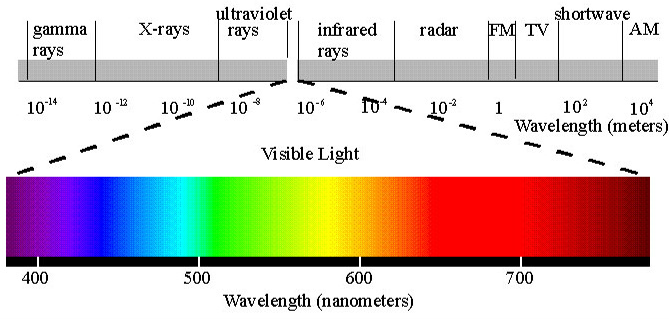
\includegraphics{./LectureNotePics/EMSpectrum.png}\unskip}
	\end{center}
\end{frame}

\section{只有波能办到的事儿}

\subsection{多普勒效应}

\begin{frame}{Doppler Effect 多普勒效应}
	\begin{itemize}
		\item 定义:当发出波的波源source或者接收波的接收器observer(或者两者同时)相对于波的传播介质运动时,接收到的波的波长和频率改变.
		\item 例子:当警车开向我们时,感觉警笛音调变高了,开过我们身边后远离我们时,感觉警笛音调变低了.
		\item 应用:交警的测速仪
	\end{itemize}
\end{frame}

\begin{frame}{Doppler Effect 多普勒效应}
	\begin{block}{多普勒效应的公式}
		\[f' = f\left(\frac{V \pm V_o}{V \pm V_s}\right)\]
	\end{block}
	
	\begin{enumerate}
		\item $f$是发出的频率,$f'$是收到的频率.
		\item $V_o$是接收器\textbf{相对于介质}的速度,$V_s$是波源\textbf{相对于介质}的速度.
		\item 最容易扣分的点:$V_o$和$V_s$的正负号搞不清。牢记一句话:\textbf{朝着彼此移动频率升高,背离彼此移动频率降低}.
		\item 如果要算的是波长,记得多普勒效应不影响波速,所以波长仍然和频率成反比.
	\end{enumerate}
\end{frame}

\subsection{干涉}

\begin{frame}{Superposition 叠加}
	\begin{itemize}
		\item 如果介质中同时存在两个波,比如:
		\begin{align*}
			y_1\left(x, t\right) &= A_1 \cos \left[k_1 \left(x + vt\right) + \phi_1\right]\\
			y_2\left(x, t\right) &= A_1 \cos \left[k_2 \left(x + vt\right) + \phi_2\right]
		\end{align*}
		
		\item 那么介质中任何一点在任何时刻实际离平衡位置的距离就是两者的叠加:$y = y_1 + y_2$.
		\item 同样的道理也适用于脉冲:事实上,$y_1\left(x, t\right)$和$y_2\left(x, t\right)$可以是任意的函数.
	\end{itemize}
\end{frame}

\begin{frame}{Interference 干涉}
	\begin{itemize}
		\item 干涉 (Interference):特指两个同频率连续行波的叠加.
		\item 介质中任一点的振动频率和参与干涉的两个同频波也一致.
		\item 每点的振幅未必相同,既取决于相对位置,也取决于两列波的phase constants.
		\item 每点的振幅都稳定(不随时间变化).
		\item 与干涉有关的题目,核心就是求出各点振幅,特别是哪里振幅最大,哪里最小(甚至为零).
	\end{itemize}
\end{frame}

\begin{frame}{干涉发生的条件}
	\begin{block}{定义}
		称符合以下条件的两列或更多列波为彼此相干的(coherent):
		\begin{enumerate}
			\item 两列波频率一致.
			\item 两列波分别的$\phi_0$可以不同,甚至可以各自随时间变化,但$\phi_0$之差必须保持恒定.
		\end{enumerate}
	\end{block}		
	
	\begin{itemize}
		\item 只有相干波在同一空间中传播,才能发生干涉.
		\item 产生相干波的常见办法:把同一波源发出的波分裂成两束.
	\end{itemize}
\end{frame}

\begin{frame}{1D Interference 一维干涉}
	\begin{itemize}
		\item 如果参与干涉的两列波沿同一直线传播,发生的干涉就是一维干涉.
		\item 驻波 (standing wave) 就是一种产生一维干涉的最简便办法,但不是唯一的办法.
	\end{itemize}
\end{frame}

\begin{frame}{Standing Wave 驻波}
	\begin{itemize}
		\item 比如一根绳子,一端固定住,另一端用手上下摇晃,绳子上的波碰到固定端被反射,就出现两列$A$、$k$、以及$v$的大小都相同,只有$v$的方向相反的波的叠加,叠加的结果就叫\textbf{驻波}.
		\item 为了方便,我们不妨设$\phi_0 = 0$
	\end{itemize}
	\begin{exampleblock}{思考题}
		\stuname 能化简$A \cos \left[k\left(x-vt\right)\right] + A \cos \left[k\left(x+vt\right)\right]$吗?\\(提示:和差角公式)
	\end{exampleblock}
\end{frame}

\begin{frame}{数学基础:和差化积}
	\begin{block}{和差角公式}
		\begin{align*}
			\cos\left(x + y\right) &= \cos x \cos y - \sin x \sin y\\
			\cos\left(x - y\right) &= \cos x \cos y + \sin x \sin y
		\end{align*}
	\end{block}
	
	\medskip	
	
	令$x = \dfrac{A + B}{2}$,$y = \dfrac{A - B}{2}$,则$A = x + y$,$B = x - y$:
	
	\medskip	
	
	\begin{block}{和差化积公式(之一)}
		\[\cos A + \cos B = 2 \cos\frac{A+B}{2} \cos \frac{A-B}{2}\]
	\end{block}
\end{frame}

\begin{frame}{Standing Wave 驻波}
	\begin{block}{驻波的数学形式}
		\[y\left(x, t\right) = 2A \cos kx \cos \omega t = A\left(x\right) \cos \omega t\]
	\end{block}
	
	\begin{itemize}
		\item 单个正弦波上,每个点的振幅都是完全相同的,都是$A$.
		\item 一旦形成驻波,各点的振幅就不一样了.
		\item 振幅为零的点叫做波节 (node).
		\item 振幅最大的点叫做波腹 (antinode).
	\end{itemize}
\end{frame}

\begin{frame}{Node and Antinode}
	\begin{block}{驻波(动画)}
	\begin{center}
		\href{run:./LectureNotePics/StandingWave.gif}{\resizebox{.5\textwidth}{!}{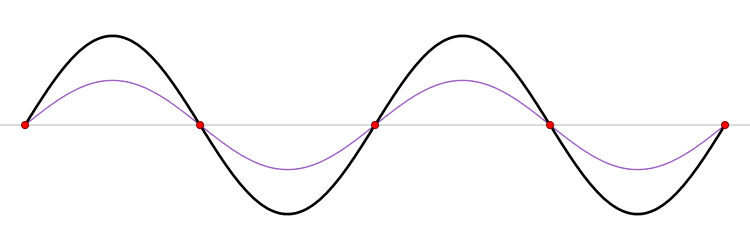
\includegraphics{./LectureNotePics/StandingWave.png}\unskip}}\\
	\end{center}
	\end{block}
	
	\begin{itemize}
		\item 节和腹交替出现.
		\item 相邻两个波腹或相邻两个波节间距半个$\lambda$.
		\item 驻波在波腹处的切线永远是平的.
	\end{itemize}
\end{frame}

\begin{frame}{一维干涉 - 同行}
	\begin{itemize}
		\item 设1号波源的位置为原点,phase constant 为零,2号波源在$x_0$处,phase constant为$\phi_0$,\textbf{\textcolor{red}{同向}}右传播,振幅相同。
		\item 写出两个波函数:
		\begin{align*}
			y_1\left(x, t\right) &= A \cos \left[kx - \omega t\right]\\
			y_2\left(x, t\right) &= A \cos \left[k\left(x - x_0\right) - \omega t + \phi_0 \right] = A \cos \left[kx - \omega t + \textcolor{red}{\phi_0 - kx_0}\right]
		\end{align*}
		
		\item 相加:
		
		\[y\left(x, t\right) = 2A \cos \frac{\phi_0 - kx_0}{2}\cos \left(kx -\omega t + \frac{\phi_0 - kx_0}{2}\right)\]
	\end{itemize}
\end{frame}

\begin{frame}{Interpretation 结果阐释}
	\begin{block}{两列同行相干波的叠加}
		\[y\left(x, t\right) = 2A \cos \frac{\phi_0 - kx_0}{2}\cos \left(kx -\omega t + \frac{\phi_0 - kx_0}{2}\right)\]
	\end{block}
	
	\begin{itemize}
		\item 仍然是一个向右传播的行波.
		\item 振幅取决于等效相差 (effective phase difference) $\phi = \phi_0 - kx_0$.
		\item 若$\phi$为偶数倍的$\pi$,振幅达最大的$2A$,这时称为\textbf{相长干涉}(constructive interference,简称CI).
		\item 若$\phi$为奇数倍的$\pi$,振幅为0,这时称为\textbf{相消干涉}(destructive interference,简称DI).
	\end{itemize}
\end{frame}

\begin{frame}{相差 Phase Difference}
	\begin{itemize}
		\item 等效相差 $\phi = \phi_0 - kx_0$.
		\item 若两个波源在同一位置,等效相差就是两者的实际相差$\phi_0$.
		\item 两波源间每隔1个波长的距离,就额外引入$2\pi$的相差.
		\item 若2号波源在1号波源的\textbf{\textcolor{red}{传播方向侧}},引入的额外相差是\textbf{\textcolor{red}{负}}的,否则是正的.
	\end{itemize}
\end{frame}

\begin{frame}{一维干涉 - 对撞}
	\begin{itemize}
		\item 1号波源在原点,phase constant 为零,向右传播;2号波源在$x_0>0$处(1号右侧),phase constant为$\phi_0$,向左传播,振幅相同。
		\item 写出两个波函数:
		\begin{align*}
			y_1\left(x, t\right) &= A \cos \left[kx - \omega t\right]\\
			y_2\left(x, t\right) &= A \cos \left[k\left(x - x_0\right) + \omega t + \phi_0 \right] = A \cos \left[kx + \omega t + \textcolor{red}{\phi_0 - kx_0}\right]
		\end{align*}
		\item 相加:
		
		\[y\left(x, t\right) = 2A \cos \left(kx + \frac{\phi_0 - kx_0}{2}\right)\cos \left(\omega t + \frac{\phi_0 - kx_0}{2}\right)\]
	\end{itemize}
\end{frame}

\begin{frame}{Interpretation 结果阐释}
	\begin{itemize}
		\item 各点振幅不同.
		\item 在固定的位置形成CI和DI.
		\item Standing wave中的CI就是波腹anti-node,DI就是波节node
	\end{itemize}
\end{frame}

\begin{frame}{Beats 差拍}
	如果两列波频率不完全相同,而是有一点儿差异,会形成所谓的beats
	\begin{block}{差拍(动画)}
	\begin{center}
		\href{run:./LectureNotePics/Beats.gif}{\resizebox{.5\textwidth}{!}{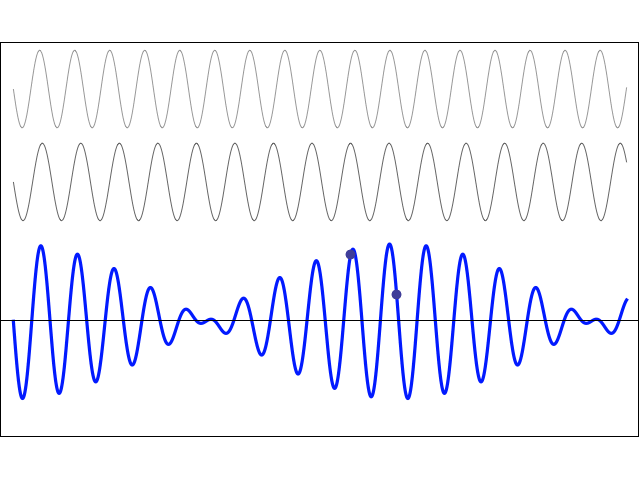
\includegraphics{./LectureNotePics/Beats.png}\unskip}}\\
	\end{center}
	\end{block}
\end{frame}

\begin{frame}{差拍的数学分析}
	\begin{itemize}
		\item 两个波源都在原点,phase constant都为零,都向右传播,振幅相同;1号波源波数是$k_1$,2号波源波数是$k_2$,$k_1-k_2<<k_2<k_1$.
		\item 写出波函数
		\begin{align*}
			y_1\left(x, t\right) &= A \cos \left[k_1\left(x - vt\right)\right]\\
			y_2\left(x, t\right) &= A \cos \left[k_2\left(x - vt\right)\right]
		\end{align*}
		\item 相加:
		
		\[y\left(x, t\right) = 2A\cos\left[\frac{k_1 + k_2}{2}\left(x - vt\right)\right]\cos\left[\frac{k_1 - k_2}{2}\left(x - vt\right)\right]\]
	\end{itemize}
\end{frame}

\begin{frame}{Interpretation 结果阐释}
	\begin{block}{一维差拍}
		\[y\left(x, t\right) = 2A\cos\left[\textcolor{red}{\frac{k_1 + k_2}{2}}\left(x - vt\right)\right]\cos\left[\textcolor{blue}{\frac{k_1 - k_2}{2}}\left(x - vt\right)\right]\]
	\end{block}
	\begin{itemize}
		\item 回忆:$f = \dfrac{v}{\lambda} = \dfrac{v}{2\pi} k$,即频率正比于波数.
		\item 红色的部分是两个$k$的平均值,因为两个$k$很接近,这个平均值也和它们很接近.
		\item 蓝色的部分非常小,描绘了一个频率很低,波长很长的波,这就是beat中振幅的缓慢变化.
		\item 请\stuname 思考:beat上一个鼓包的宽度是多少?
	\end{itemize}
\end{frame}

\end{document}
